\documentclass[a4paper,12pt]{article}
\usepackage[paper=a4paper,left=35mm,right=25mm,top=25mm,bottom=20mm]{geometry}
\usepackage[ngerman]{babel}
\usepackage[utf8]{inputenc}
\usepackage{amsmath}
\usepackage{amssymb}
\usepackage{tikz}
\usepackage{pgfplots}
\usepackage{enumitem}
\usepackage{cite}
\usepackage[square,sort,comma,numbers]{natbib}
\usepackage{graphicx}
\usepackage{float}

\linespread{1.5}

\addto\captionsngerman{
  \renewcommand{\contentsname}
    {INHALTSVERZEICHNIS}
}

\newcommand{\code}{\texttt}

\begin{document}
\parindent0cm
\setlength{\abovedisplayskip}{-1cm}
\setlength{\belowdisplayskip}{0.75cm}

%===================================================================================
%---------------------------- TITELSEITE -------------------------------------------
%===================================================================================

\thispagestyle{empty}

\begin{center}

\begin{large} 
GYMNASIUM OTTOBRUNN	\\
\vspace{1cm}
Oberstufenjahrgang 2017/19\\
\vspace{1cm}
Seminarfach Softwareentwicklung\\
\vspace{2cm}
Seminararbeit\\
\end{large}


\vspace{1cm}


{\Huge\bfseries 
36. Bundeswettbewerb Informatik\par
Runde 2\par
Aufgabe 1 und 3\par 
}


\vspace{2cm}


\begin{large}
\begin{tabular}{rl}
Verfasser:& Jonas Fritsch \\
Seminarleiter: & StD Peter Brichzin \\
Bewertung:  & ......... Punkte  \\
Unterschrift des Seminarleiters: & ...........................................  \\
\end{tabular} 
\end{large}

\end{center}

%===================================================================================
%---------------------------- INHALTSVERZEICHNIS -----------------------------------
%===================================================================================				

\newpage

\thispagestyle{empty}
\tableofcontents	
\thispagestyle{empty}



%===================================================================================
%-------------------------------- EINLEITUNG ---------------------------------------
%===================================================================================

\newpage
\setcounter{page}{4}
\section{EINLEITUNG}



Der aus drei Runden bestehende Bundeswettbewerb Informatik (BwInf) ist einer von vier Bundesweiten Informatikwettbewerben. Mit dem 36. BwInf wurde für die erste Runde mit \textbf{1463} Teilnehmern eine so hohe Teilnahme wie seit 1993 nicht mehr geschafft \cite{bwinf_runde1_ergebnis}. Von den ursprünglich 1463 Teilnehmern der ersten Runde, haben es \textbf{828} Teilnehmende geschafft sich für die zweite Runde zu qualifizieren \cite{bwinf_runde2_ergebnis}. Von diesen haben jedoch nur noch \textbf{154} Teilnehmer der zweiten Runde Lösungen für zwei Aufgaben ihrer Wahl eingereicht. Dies liegt nicht zuletzt an der stark steigenden Komplexität der Aufgaben gegenüber der ersten Runde. Zu der letzten, dritten Runde des Bundeswettbewerbs Informatik werden schlussendlich nur noch \textbf{25} Teilnehmer eingeladen. Das sind im Falle des BwInfs von 2017 nur rund \textbf{1,7\%} der ursprünglichen Teilnehmer.
\\[0.4cm]
Im Folgenden wird eine eingereichte Lösung zu der ersten und dritten Aufgabe der zweiten Runde des 36. Bundeswettbewerbs Informatik erläutert.

%===================================================================================
%-------------------------------- AUFGABE 1 ----------------------------------------
%===================================================================================

\newpage
\section{AUFGABE 1 - "Die Kunst der Fuge"}



\subsection{Aufgabenstellung}
Ilona besitzt einen riesigen Haufen Holzklötzchen: Diese haben alle dieselbe Höhe und Tiefe,
aber verschiedene Längen. \\
Ilona möchte eine Mauer bauen. Jede Reihe der Mauer soll aus $n$ Klötzchen bestehen, die die
Längen 1 bis $n$ haben und lückenlos aneinander liegen. Die Stellen zwischen den Klötzchen heißen
Fugen. Ilona möchte, dass in der fertigen Mauer niemals zwei Fugen übereinander liegen,
selbst wenn sich mehrere Reihen dazwischen befinden. Außerdem soll ihre Mauer möglichst
hoch sein. \\
Für $n = 4$ gelingt es ihr recht schnell, eine Mauer mit drei Reihen zu bauen:
\begin{figure}[H]
    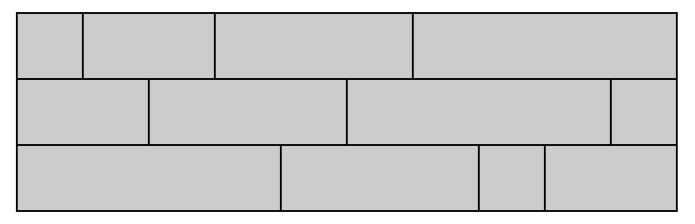
\includegraphics[width=0.7\linewidth]{Bilder/Aufgabe1/Aufgabenstellung_BeispielMauer.png}
\end{figure}
\begin{large}
    \textbf{Aufgabe} \\
\end{large}
Hilf Ilona, indem du ein Programm schreibst, das nach Eingabe von $n$ eine nach ihren Vorgaben
konstruierte, möglichst hohe Mauer ausgibt. Für $n = 10$ sollte dein Programm eine Mauer der
Höhe 6 ausgeben können. Wie hoch werden die Mauern deines Programms für größere $n$?

\subsection{Auslegung der Aufgabe}
Die grundlegende Aufgabe ist, eine Mauer mit möglichst vielen Reihen, die aus verschieden länglichen Klötzchen bestehen, zu bauen.

Die Längen der Klötzchen in einer Reihe sind durch eine Variable $n$ definiert.
Die Variable $n$ ($n \in \mathbb{N}$\textbackslash$\{0\}$) definiert dabei die Längen und auch die Gesamtanzahl der Klötzchen pro Reihe.
Gesamtanzahl heißt, dass bei zum Beispiel $n = 5$ jede Reihe aus 5 einzelnen Klötzchen besteht. 
Jede Reihe setzt sich dann aus einem 1er, einem 2er, einem 3er, einem 4er und einem 5er Klotz zusammen.
\\[0.4cm]
Der Trick bei der Aufgabe ist nun, dass niemals zwei Fugen \textbf{übereinanderliegen dürfen}.
Eine Fuge ist die Lücke zwischen zwei Klötzchen (siehe Abbildung 1).
\begin{figure}[H]
    \centering
    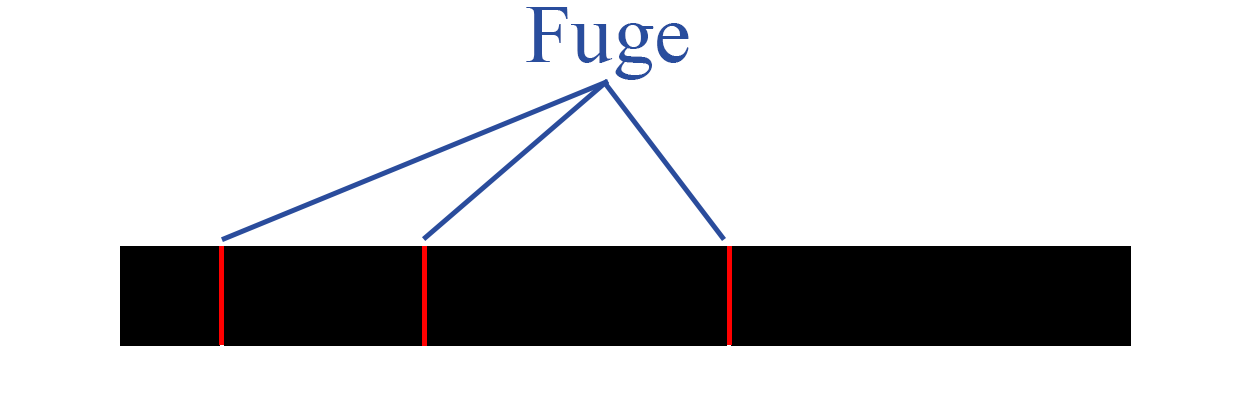
\includegraphics[width=0.8\linewidth]{Bilder/Aufgabe1/Definition_Fuge.png}
    \caption{Darstellung der 3 Fugen einer Reihe mit 4 Klötzchen}
\end{figure}

Als Hilfestellung wurde außerdem erwähnt, dass eine Mauer für $n = 10$ eine maximale Höhe von $6$ hat.

\subsection{Lösungsidee}
\subsubsection{Verstehen des Problems}
Um die Problemstellung der Aufgabe genauer zu verstehen, bietet es sich erstmal an, Mauern für kleinere $n$ auf Papier zu zeichnen.
Beginnt man mit $n = 1$, fällt auf, dass ganz gleich wie viele Reihen übereinanderliegen, es nie zu einer Fugenüberlappung kommen kann, da eine Reihe mit einem einzelnen Klötzchen keine Fuge besitzt.
Für $n = 1$ kann also theoretisch eine \textbf{unendlich} hohe Mauer gebaut werden.
\\[0.4cm]
Für $n = 2$ ist es auch noch recht einfach, eine Mauer zu bauen. Denn es gibt pro Reihe nur 2 mögliche Reihenfolgen von Klötzchen. Entweder kommt zuerst der 1er oder der 2er Klotz. 
Eine der zwei möglichen Lösungen ist in Abbildung 2 zu sehen. Es gibt keine Möglichkeit, noch ein Klötzchen in einer neuen dritten Reihe zu platzieren, ohne eine Fuge doppelt zu besetzen.
\begin{figure}[H]
    \centering
    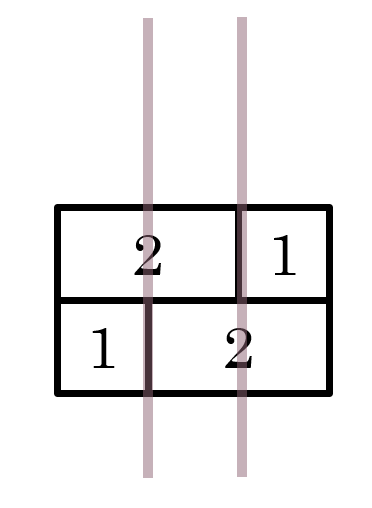
\includegraphics[width=0.25\linewidth]{Bilder/Aufgabe1/Loesung_N2.png}
    \caption{Eine der zwei möglichen Lösungen für $n = 2$. Die roten Striche zeigen an, dass die jeweilige Fuge bereits besetzt ist.}
\end{figure}

Auch für $n = 3$ gibt es eine Mauer mit einer maximalen Höhe von 2 (siehe Abbildung 3). Hier wird es jedoch schon komplexer, da es nun für eine Reihe nicht mehr $2! = 2\times1 = 2$, sondern $3! = 3\times2\times1 = 6$ mögliche Klötzchen-Reihenfolgen gibt.
Außerdem tritt bei $N = 3$ das erste Mal auf, dass eine \textbf{mögliche Fugenstelle nicht besetzt wird.}
\begin{figure}[H]
    \centering
    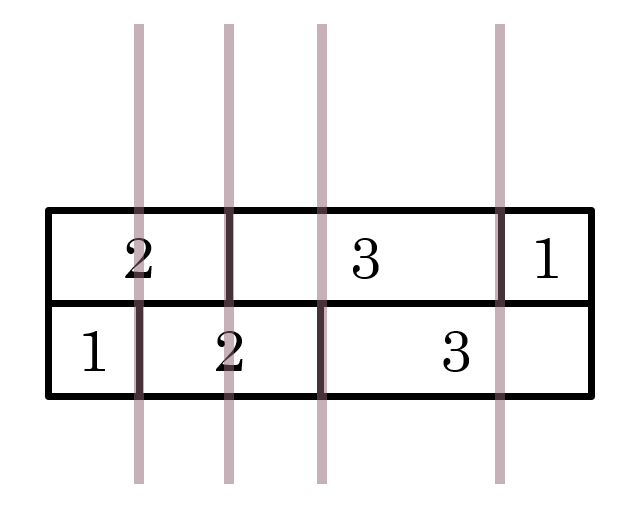
\includegraphics[width=0.4\linewidth]{Bilder/Aufgabe1/Loesung_N3.png}
    \caption{Eine mögliche Lösung für $n = 3$. Zu beachten ist, dass in der Mauer eine \textbf{mögliche} Fugenstelle, dort wo es eine größere Lücke zwischen den zwei letzten besetzten Fugenstellen gibt, \textbf{unbesetzt bleibt.}}
\end{figure}

Geht man noch weiter und bildet eine Mauer für $n = 4$ ($4! = 24$ mögliche Klötzchen Anordnungen pro Reihe), so kann man erstmals eine Mauer der Höhe 3 bilden (siehe Abbildung 4). Hier ist auch wieder jede einzelne Fugenstelle besetzt.
\begin{figure}[H]
    \centering
    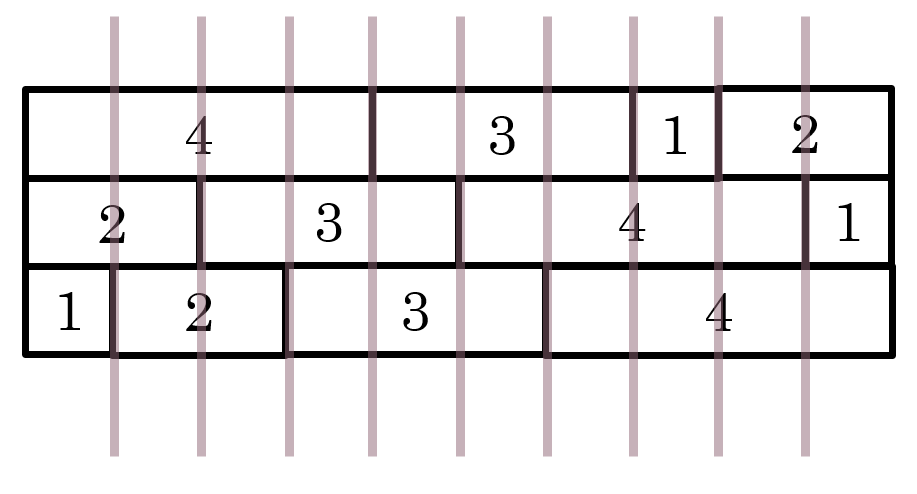
\includegraphics[width=0.6\linewidth]{Bilder/Aufgabe1/Loesung_N4.png}
    \caption{Eine mögliche Lösung für $n = 4$}
\end{figure}

Die Komplexität der Aufgabe steigt mit höheren $n$ stark an. Während man bei $n = 2$ $2!$ Möglichkeiten pro Reihe und 2 Reihen hatte ($2!\times2 = 4$ unterschiedliche Mauern), gibt es bei $n = 4$ bereits $4!\times3 = 72$ verschiedene Mauern.
Allgemein gibt es also für eine Mauer $n!\times h$ Lösungen, wobei $h$ die Anzahl der übereinanderliegenden Reihen ist.
\\[0.4cm]
Es ist logisch, dass zwischen der Anzahl der maximal möglichen Reihen $h$ und der Anzahl der Klötzchen pro Reihe $n$ eine Abhängigkeit existiert.
\\[0.4cm]
Allgemein kann man sagen, dass die \textbf{maximale Mauerhöhe} dann erreicht ist, wenn \textbf{nicht} mehr \textbf{genug Fugenstellen in der Mauer frei sind}, um eine \textbf{weitere Reihe zu bilden}.

Somit lässt sich die Formel
\begin{center}
\begin{Large}
\[h = \frac{f_{Mauer}}{f_{Reihe}}\]
\end{Large}
\end{center}
ableiten, wobei $f_{Mauer}$ die maximale Anzahl an Fugen in der Mauer und $f_{Reihe}$ die Anzahl der Fugen, die eine Reihe besetzt, beschreibt.
\\[0.4cm]
Um nun auf $f_{Mauer}$ schließen zu können, braucht man nur die Länge der Mauer. Da jede Reihe der Mauer gleich lang ist, ist die Länge der Mauer gleich der Länge einer Reihe. Die Länge einer Reihe definiert sich wiederum durch die Menge und Breite ihrer Klötzchen. Das heißt also, die Länge einer Reihe/der Mauer ist nach der \textbf{Gaußschen Summenformel}
% TODO: Quelle für Gaußsche Summenformel
\begin{center}
\begin{Large}
\[1+2...+n = \sum_{k=1}^n k = \frac{n(n+1)}{2}\]
\end{Large}
\end{center}
Um nun aber von der Länge der Mauer auf $f_{Mauer}$ zu kommen, muss man noch $1$ von der Länge der Mauer abziehen. Dies wird offensichtlich, wenn man zu einer Mauer eine Reihe aus lauter 1er Klötzchen bildet (siehe Abbildung 5). Da das Ende des letzten Klötzchens nicht als Fuge gilt, wird von der Länge der Reihe noch $1$ abgezogen.
\begin{figure}[H]
    \centering
    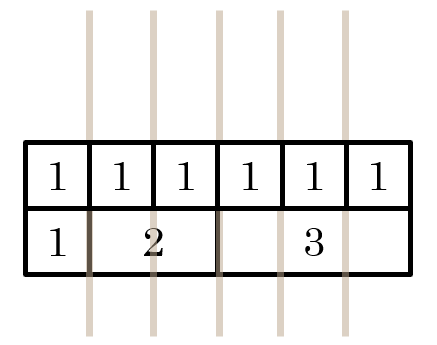
\includegraphics[width=0.4\linewidth]{Bilder/Aufgabe1/Definition_Fugenstellen_Mauer.png}
    \caption{Eine Mauer der Länge 6 besitzt 5 mögliche Fugenstellen.}
\end{figure}

Ähnlich lässt sich auch $f_{Reihe}$ berechnen. Um wissen zu wollen, wie viele freie Fugen eine Reihe mit $n$ Klötzchen besetzen wird, zieht man einfach wieder 1 von der Anzahl der Klötzchen pro Reihe ($n$) ab (siehe Abbildung 6).
\begin{figure}[H]
    \centering
    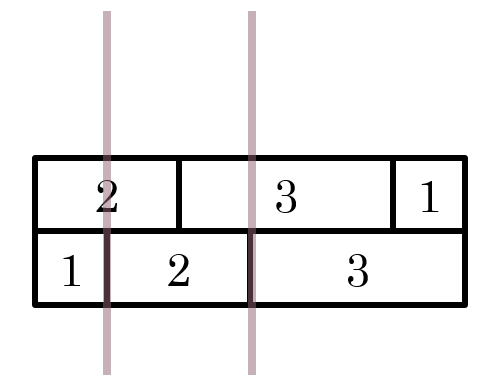
\includegraphics[width=0.4\linewidth]{Bilder/Aufgabe1/Definition_Fugenstellen_Reihe.png}
    \caption{Eine Reihe bei $n = 3$ besetzt $n-1 = 2$ freie Fugen.}
\end{figure}

Daraus ergibt sich die fertige Formel für die Anzahl der Reihen $h$ in einer maximal hohen Mauer in Abhängigkeit von $n$.
\begin{center}
\begin{Large}
\[h = \frac{\frac{n\times(n+1)}{2}-1}{n-1} = \frac{n}{2}+1\]
\end{Large}
\end{center}

Der Graph der daraus folgenden Funktion $h(n) = \frac{n}{2}+1$ verläuft dabei linear (siehe Abbildung 7).
\begin{figure}[H]
    \centering
    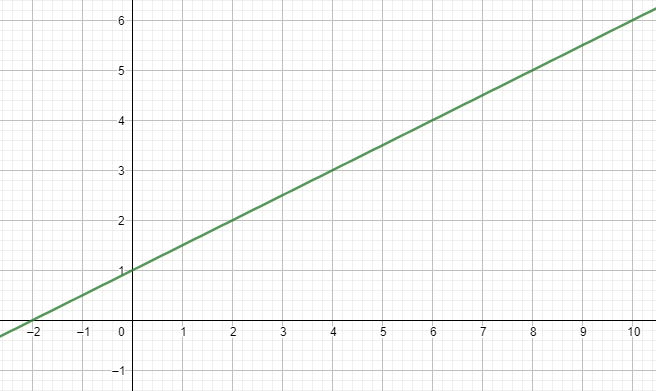
\includegraphics[width=0.95\linewidth]{Bilder/Aufgabe1/Graph_01.png}
    \caption{Graph der linearen Funktion $h(n) = \frac{n}{2}+1$}
\end{figure}
Setzt man nun für $n = 10$ ein, kommt der Funktionswert $6$ raus der mit der in der Aufgabenstellung angegebenen Höhe für eine Mauer von $n = 10$ übereinstimmt.
Testet man allerdings die maximale Mauerhöhe für zum Beispiel $n = 3$, so kommt als Wert ungefähr $2,5$ raus. Dies macht allerdings keinen Sinn, da die fertige Mauer nur aus vollen Reihen bestehen muss und keine halbfertige Mauer besitzen kann.
\\[0.4cm]
Diese Komma-Werte kommen bei allen ungeraden $n$ vor. Der Zusammenhang ist dabei, das wie beim vorherigen Beispiel $n = 3$ (siehe Abbildung 3) eine Fuge unbesetzt bleibt. Diese Fuge kann zwar mit einem weiteren Klotz besetzt werden, die Reihe könnte aber nicht mehr vollständig gebaut werden.
Da unsere Mauerhöhe also eine Natürliche Zahl sein muss, umgeben wir den Funktionsterm noch mit Abrundungsklammern:
\begin{center}
\begin{Large}
\[h(n) = \lfloor\frac{n}{2}+1\rfloor\]
\end{Large}
\end{center}
Der daraus resultierende Graph ist in Abbildung 8 zu sehen.
\begin{figure}[H]
    \centering
    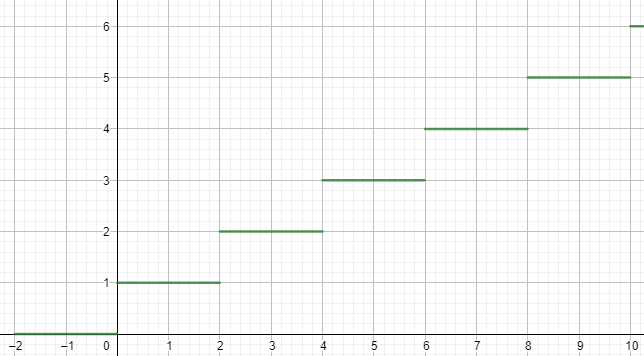
\includegraphics[width=0.95\linewidth]{Bilder/Aufgabe1/Graph_02.png}
    \caption{Graph der Funktion $h(n) = \lfloor\frac{n}{2}+1\rfloor$}
\end{figure}
Somit gibt uns die Funktion $h(n)$ mit der Definitionsmenge $\mathbb{D}_{h} = \mathbb{N}$\textbackslash$\{0;1\}$ und der Wertemenge $\mathbb{W}_{h} = \mathbb{N}$\textbackslash$\{0\}$ die jeweilige maximale Mauerhöhe ($h$) in Abhängigkeit von $n$ an. Wobei in der Definitionsmenge auch $1$ ausgeschlossen ist, weil für $n = 1$ aus logischer Sicht eine unendlich hohe Mauer und nicht nur eine Mauer der Höhe 1 gebildet werden kann.
\\[0.4cm]
Die naivste Lösung für die Aufgabe wäre per Brute-Force so lange Klötzchen aneinanderzureihen und Reihen aufeinanderzustapeln, bis man eine fertige Mauer der maximalen Höhe erreicht hat.
\\[0.4cm]
Für die in der Aufgabenstellung festgelegte Mindestanforderung $n = 10$, gäbe es bereits
\begin{center}
\begin{Large}
\[f(10) = 10!^6\approx2,28\mathrm{e}{+39}\]
\end{Large}
\end{center}
\textbf{unterschiedliche Mauerkombinationen} bei der maximalen Mauerhöhe von 6.
Der Graph der allgemeinen Formel
\begin{center}
\begin{Large}
\[f(n) = n!^{\lfloor\frac{n}{2}+1\rfloor}\]
\end{Large}
\end{center}
ist in Abbildung 9 zu sehen.
\begin{figure}[H]
    \centering
    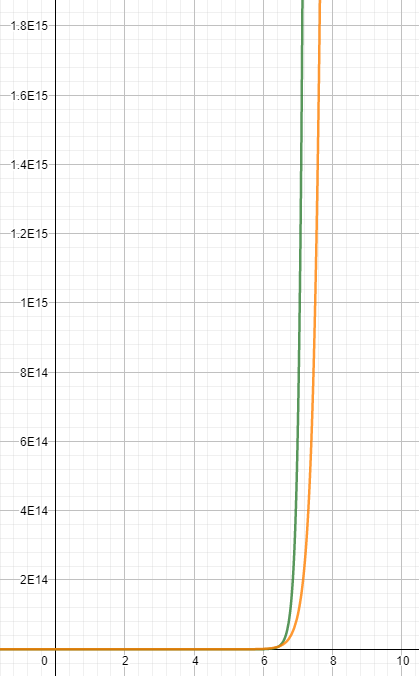
\includegraphics[width=0.7\linewidth]{Bilder/Aufgabe1/Graph_03.png}
    \caption{Der grüne Graph zeigt die extreme Steigung der Funktion 
        $f(n) = n!^{\lfloor\frac{n}{2}+1\rfloor}$. Zum Vergleich der orangen-farbige Graph der Funktion $g(x) = 100^{x}$.}
\end{figure}
Die Anzahl der verschiedenen möglichen Mauern für $n$ steigt somit mehr als 
\textbf{exponentiell}.
\\[0.4cm]
Nun ist hierbei zwar zu beachten, dass es durchaus mehrere mögliche unterschiedliche Lösungen geben kann und das bei der Gesamtmenge unterschiedlicher Mauern auch auf die Reihenfolge von Reihen geachtet wird (siehe Abbildung 10), welche für die Aufgabenstellung keinen Unterschied macht.
\begin{figure}[H]
    \centering
    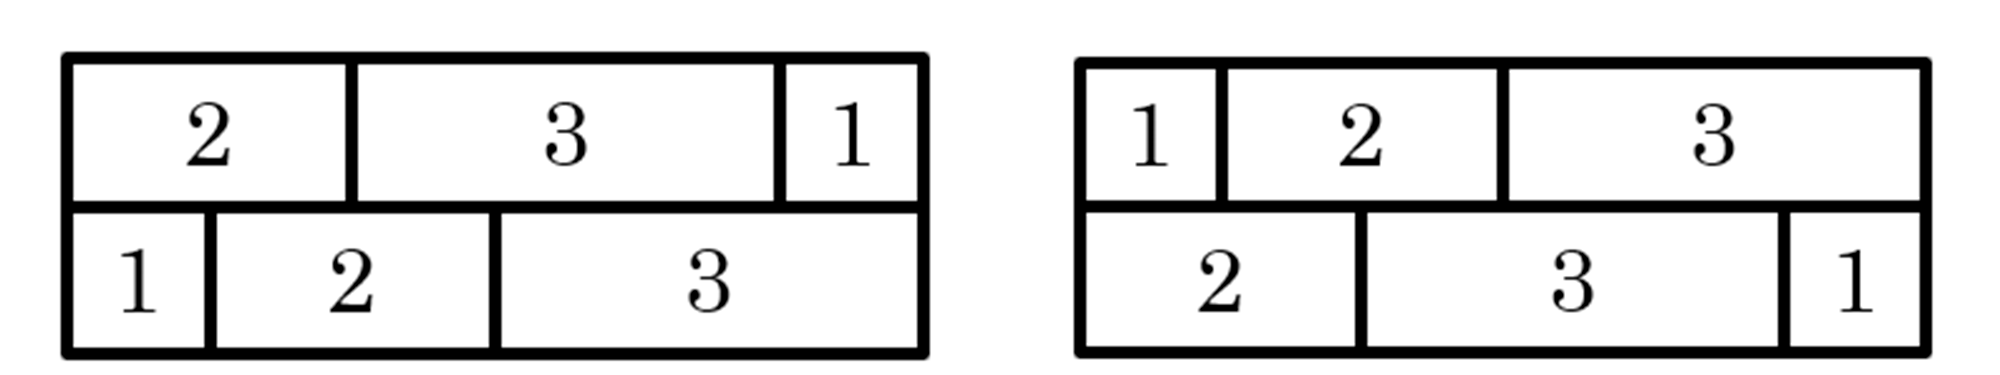
\includegraphics[width=0.9\linewidth]{Bilder/Aufgabe1/Mauervarianten_N3.png}
    \caption{Obwohl beide Mauern aus den selben zwei Reihen bestehen, werden sie als unterschiedliche Mauern angesehen.}
\end{figure}
Weiterhin ist zu beachten, dass es für Mauern mit ungeradem $n$ mehr unterschiedliche Lösungen gibt, als für die wieder darauffolgende Mauer mit geradem $n$.

Dies liegt eben daran, dass bei ungeraden $n$ immer mindestens eine Fugenstelle frei bleibt, was wiederum zu mehr richtigen Mauervariationen führt.
\\[0.4cm]
Trotzdem würde das Finden einer Lösung für $n = 10$, selbst wenn ein Computer nur \textbf{1 Millisekunde} für die Permutation einer \textbf{gesamten Mauer} benötigen würde, die maximal erwartete Algorithmuslaufzeit einer BwInf-Lösung bei weitem überschreiten.
\\[0.4cm]
Damit ist eine naive Brute-Force Methode als Lösung ausgeschlossen und es muss nach einem effizienteren Algorithmus gesucht werden.

\subsubsection{Der Algorithmus}
Grundlegend gibt es zwei unterschiedliche Wege eine Mauer, wie in der Aufgabenstellung zu bauen.
\\[0.4cm]
Der offensichtlichere ist die Bauart \textbf{'von unten nach oben'}. Bei dieser Bauart setzt man zuerst die Klötzchen zu einer Reihe zusammen. Hat man eine Reihe fertig, beginnt man mit der zweiten Reihe und so weiter (siehe Abbildung 11). Man setzt Reihe auf Reihe (von unten nach oben) bis man die Maximalhöhe erreicht hat.
\begin{figure}[H]
    \centering
    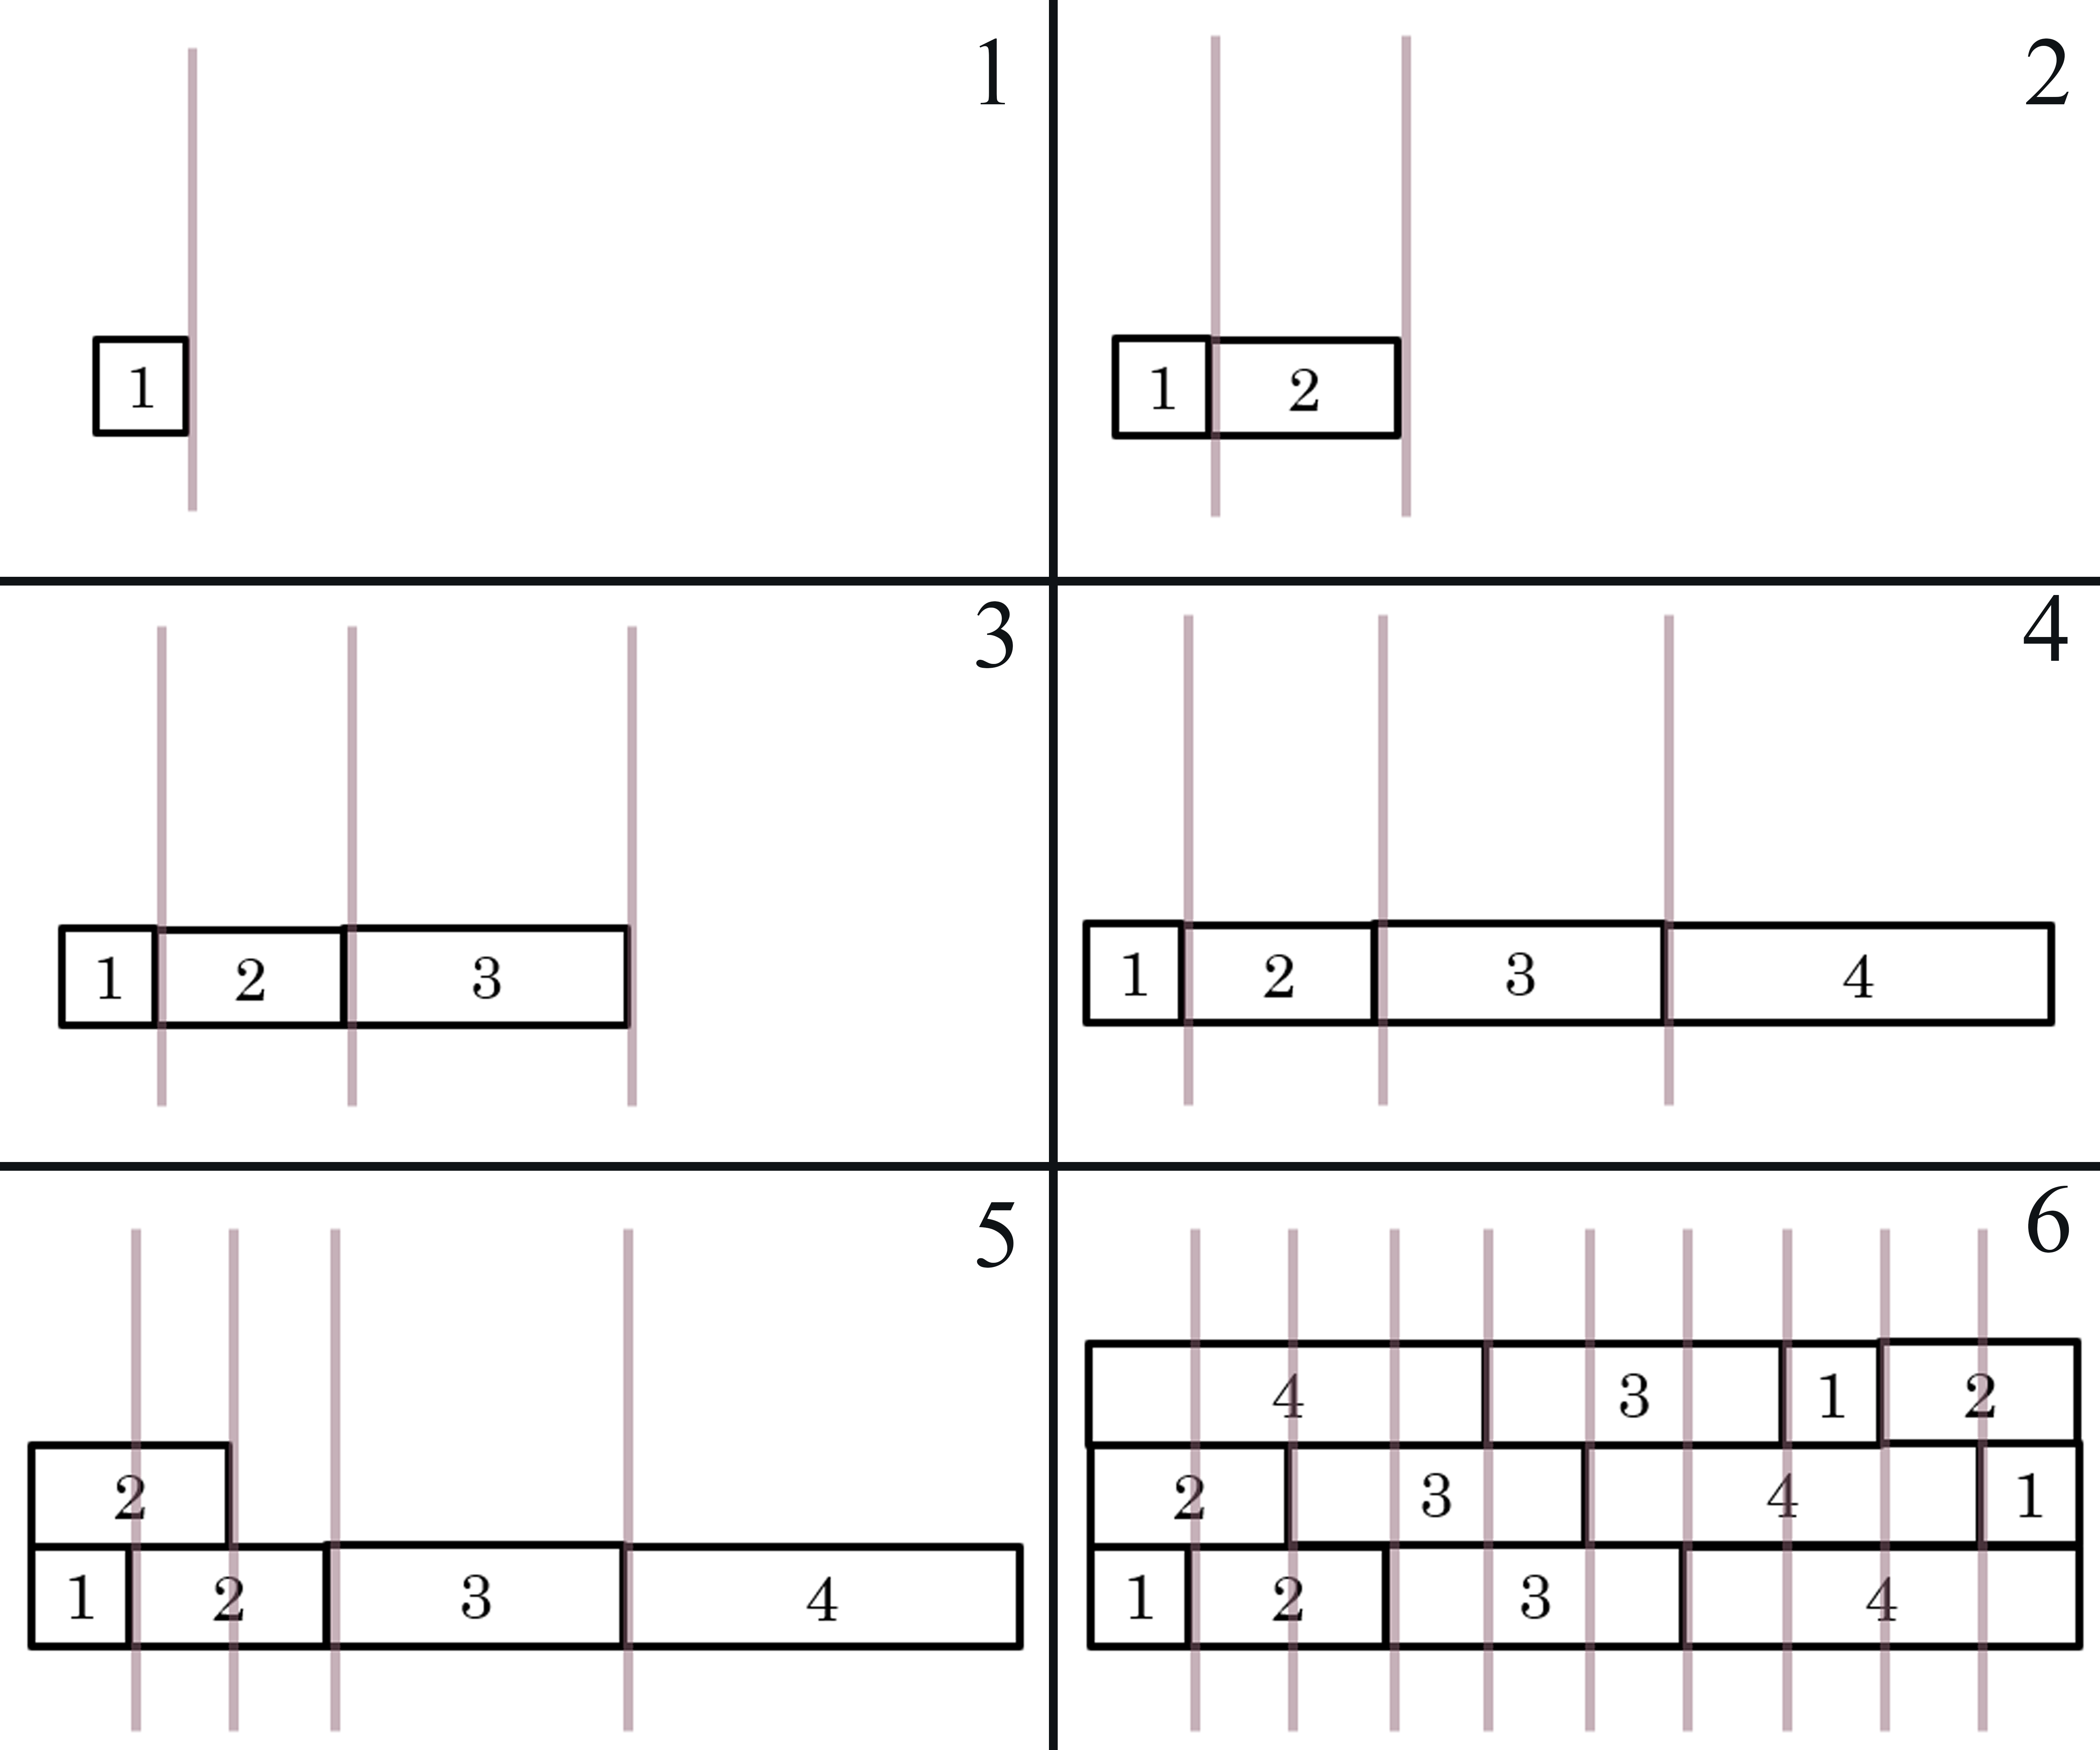
\includegraphics[width=1\linewidth]{Bilder/Aufgabe1/Definition_Mauerbauart_01.png}
    \caption{Der Bau einer Mauer nach der \textbf{'von unten nach oben'} Methode. Es wird Reihe nach Reihe gebaut (1-5), bis die maximale Höhe erreicht wurde (6).}
\end{figure}

Eine andere Möglichkeit ist, wenn man die Anzahl der Reihen ($h$) für eine Mauer der maximalen Höhe bereits weiß, die Mauer \textbf{'von links nach rechts'} aufzubauen.
Man kann die Aufgabe auch so formulieren, dass das \textbf{Ziel ist, möglichst alle Fugenposition in der Mauer zu füllen}. Nun bietet es sich an, anstatt wie bei \textbf{'von unten nach oben'} immer einen Klotz zu setzen und \textbf{dann} zu gucken, ob die jeweilige Fugenposition noch frei ist, von den \textbf{Fugenpositionen auszugehen} und diese jeweils zu versuchen \textbf{mit einem Klotz zu füllen} (siehe Abbildung 12).
\begin{figure}[H]
    \centering
    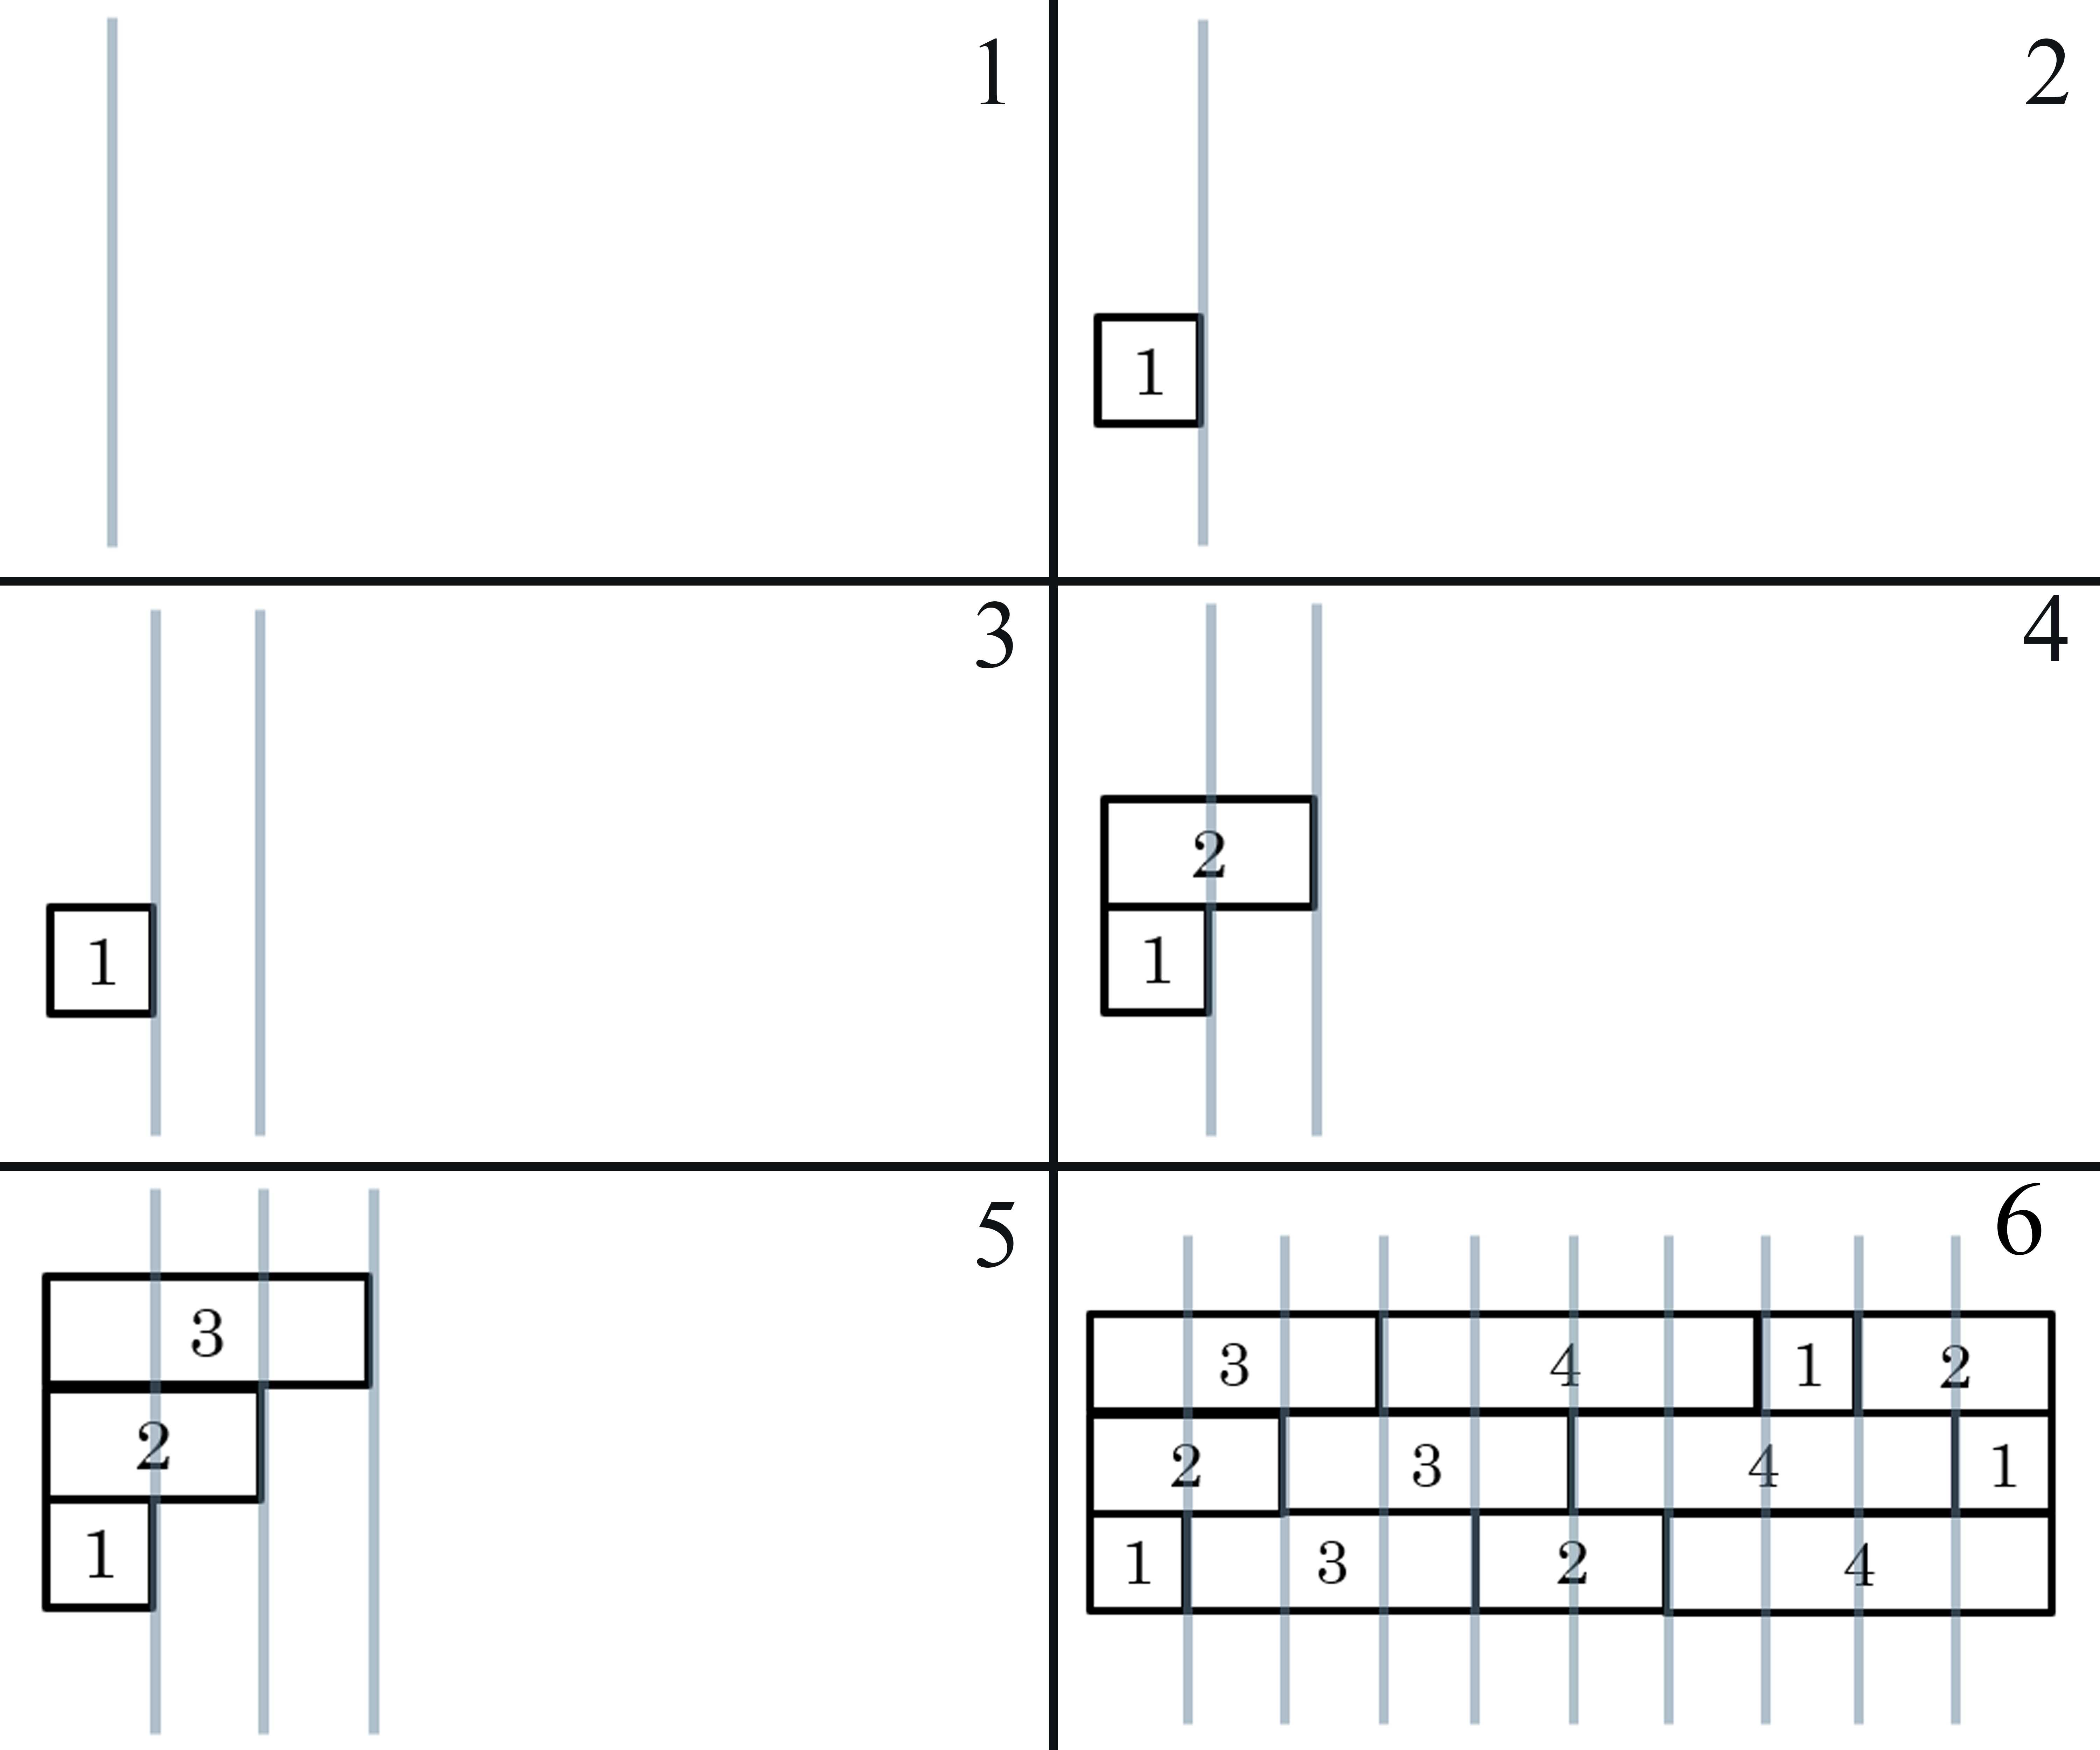
\includegraphics[width=1\linewidth]{Bilder/Aufgabe1/Definition_Mauerbauart_02.png}
    \caption{Der Bau einer Mauer nach der \textbf{'von links nach rechts'} Methode. Es wird jeweils immer die nächste freie Fuge angeschaut und überprüft, welcher Klotz in welcher Reihe diese Fuge füllen kann. Dieser Klotz wird dann gesetzt (1-5). Dies wiederholt sich solange, bis die letzte Fuge erreicht wurde und die Mauer fertig ist (6).}
\end{figure}

Diese \textbf{"Von links nach rechts"}-Bauart ist dadurch möglich geworden, dass man schon im vornherein die Anzahl an Reihen weiß, die für eine maximale Mauer benötigt wird.

Aber auch bei dieser Bauart bleibt die Frage, was passiert, wenn mehr als ein Klotz die nächste Fuge füllen kann. Dies passiert nämlich bei fast jeder Fuge (siehe Abbildung 13).
\begin{figure}[H]
    \centering
    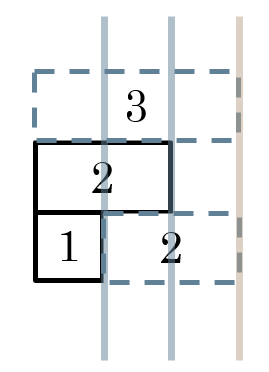
\includegraphics[width=0.3\linewidth]{Bilder/Aufgabe1/Problem_Mauerbauart_02_Mehrere_Kloetze.png}
    \caption{Zum Besetzen der dritten Fuge (orange markiert) bei $n = 4$ kann entweder ein 3er Klötzchen in einer neuen Reihe, oder ein 2er Klötzchen in der untersten Reihe platziert werden.}
\end{figure}

Wählt man ein zufälliges Klötzchen aus, so kann es schnell dazu kommen, dass eine Reihe soweit in 'Rückstand' gerät, dass kein möglicher Klotz mehr lang genug wäre, um die Reihe fortzuführen (siehe Abbildung 14).
\begin{figure}[H]
    \centering
    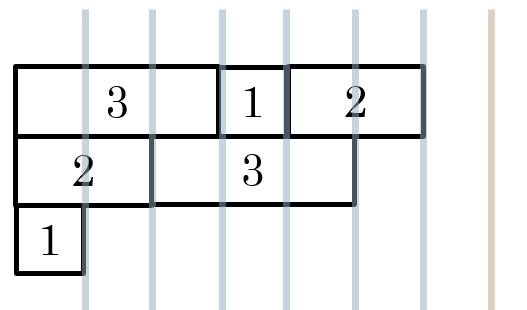
\includegraphics[width=0.5\linewidth]{Bilder/Aufgabe1/Problem_Mauerbauart_02_RowSum.png}
    \caption{In der dargestellten Mauer für $n = 4$, gibt es für die \textbf{unterste Reihe keine Möglichkeit mehr ein Klötzchen zu platzieren}. Da die obereren Reihen alle Fugen schon besetzt haben und die nächste freie Fuge \textbf{6 Längen} von der untersten Reihe entfernt ist, würde diese Reihe ein \textbf{6er Klötzchen} benötigen. Bei $n = 4$ gibt es jedoch maximal \textbf{4er Klötzchen}.}
\end{figure}
Es ist also wichtig immer darauf zu achten, dass die kürzeste Reihe nicht den Anschluss verliert.
\\[0.4cm]
Die Lösung für dieses Problem ist bei dem Fall, dass wenn verschiedene Klötzchen mehrerer Reihen eine Fuge befüllen können, immer die \textbf{kürzeste Reihe zu bevorzugen}.
\\[0.4cm]
Mit diesem Algorithmus kommt man bis zu $n = 8$. Dort tritt ein weiteres Problem auf (siehe Abbildung 15).
\begin{figure}[H]
    \centering
    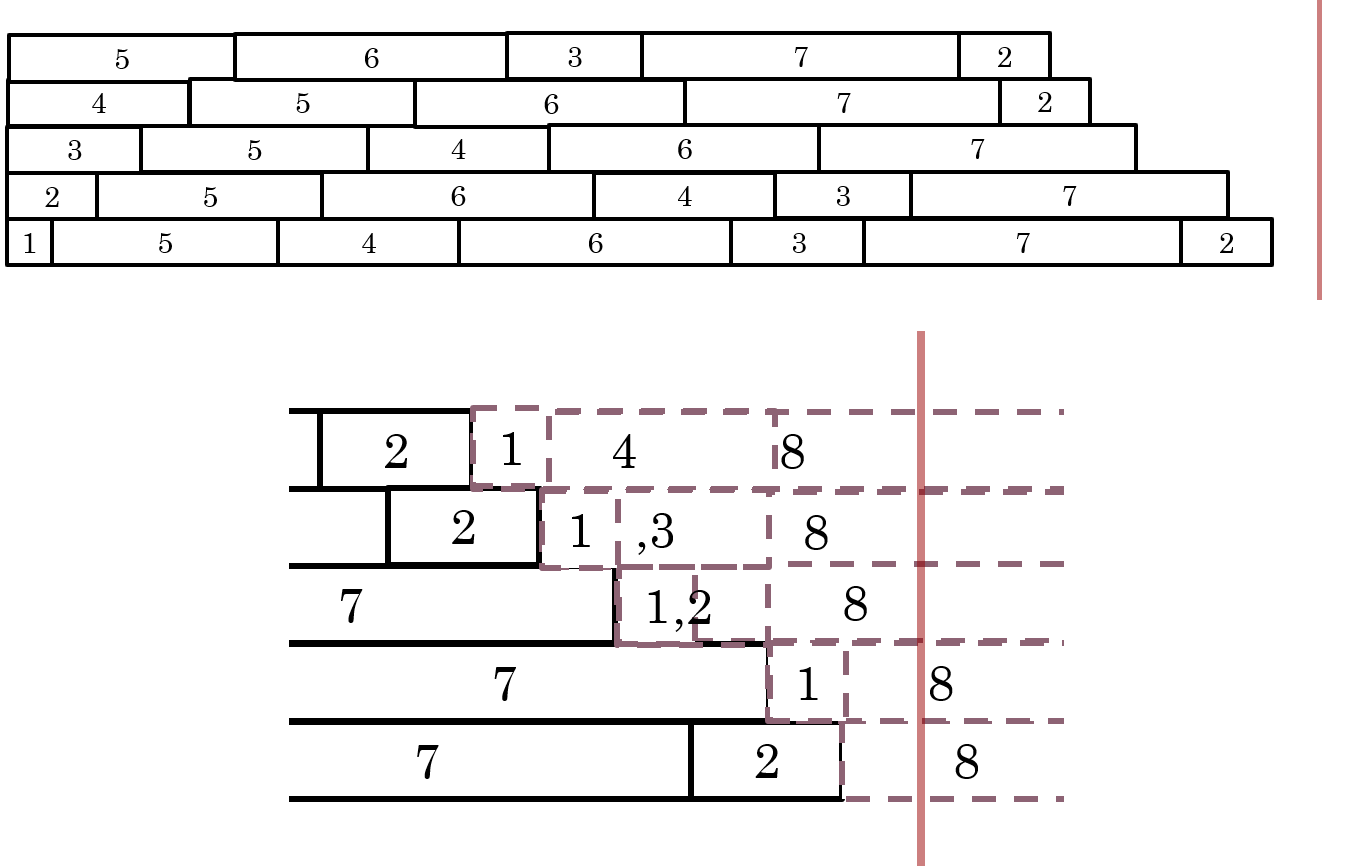
\includegraphics[width=1\linewidth]{Bilder/Aufgabe1/Problem_Mauerbauart_02_Kein_Klotz.png}
    \caption{Bei $n = 8$ tritt das Problem auf, dass die \textbf{29 Fuge} (rot markiert), durch \textbf{kein einziges, mögliches Klötzchen besetzt werden kann}. Da $n$ jedoch eine \textbf{gerade Zahl} ist, wissen wir, dass für eine Mauer der maximalen Höhe \textbf{alle Fugen besetzt werden müssen}. Das untere Bild zeigt nochmal den hinteren Ausschnitt der Mauer mit allen noch möglichen Klötzchen für jede Reihe an. Keines davon würde die nächste Lücke füllen.}
\end{figure}
%TODO: Quelle für Backtracking
Um dennoch eine Lösung zu bekommen, wird \textbf{Backtracking} verwendet. Backtracking erlaubt es, \textbf{zur letzten Entscheidung zurückzugehen} und eben \textbf{eine andere} zu \textbf{treffen}. Mit "Entscheidung" ist die Wahl eines Klötzchens um eine freie Fuge zu besetzen, wenn es mehrere Möglichkeiten gäbe gemeint (siehe Abbildung 16).
\begin{figure}[H]
    \centering
    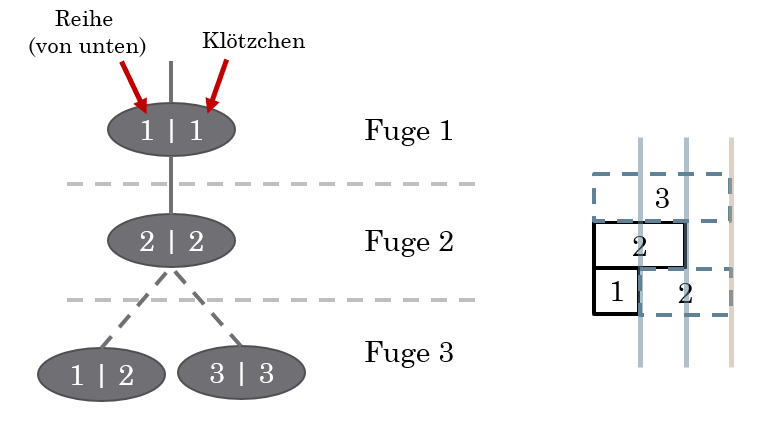
\includegraphics[width=1\linewidth]{Bilder/Aufgabe1/Backtracking_01.png}
    \caption{Bei einer Mauer von $n = 4$ tritt das vorher schon besprochene Problem auf, dass es zwei mögliche Klötzchen gibt, die die \textbf{3 Fuge} besetzen können. Der Baum auf der linken Seite veranschaulicht die möglichen Klötzchen pro Fuge. Die \textbf{Tiefe des Baumes} entspricht dabei einer \textbf{jeweiligen Fugenposition} und die \textbf{Knoten dieser Tiefe} stehen für die \textbf{möglichen Klötzchen}.}
\end{figure}
Wählen wir nun das Klötzchen der kürzesten Reihe (das 3er Klötzchen in der obersten, neuen Reihe) und \textbf{gehen davon aus, dass die 4te Fuge nun nicht mehr gefüllt werden kann} (siehe Abbildung 17),
\begin{figure}[H]
    \centering
    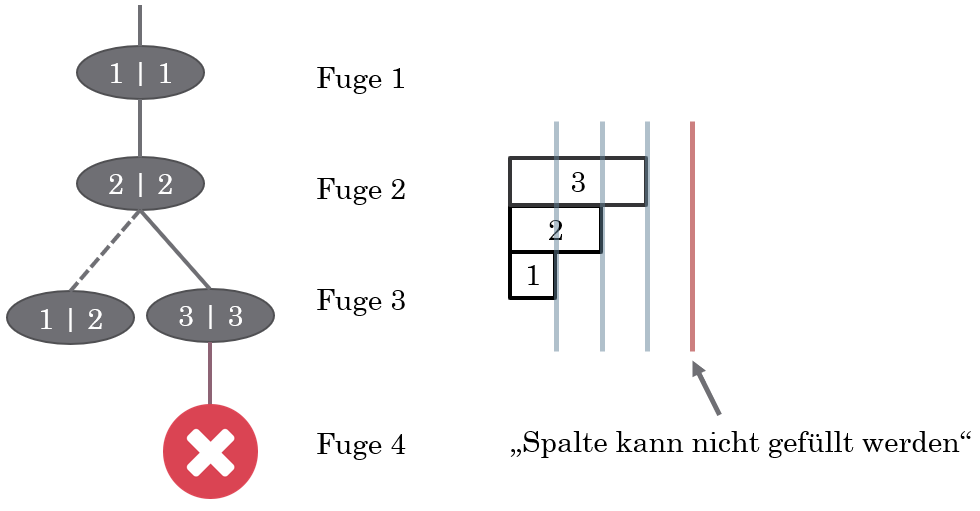
\includegraphics[width=1\linewidth]{Bilder/Aufgabe1/Backtracking_02.png}
    \caption{Angenommen nach der Entscheidung vom einsetzen des 3er Klötzchens, kann die 4te freie Fuge nicht besetzt werden. Theoretisch könnte in der untersten Reihe ein 3er Klotz die 4te Fuge füllen. Zur Vereinfachung der Darstellung wird dies jedoch außer Acht gelassen.}
\end{figure}
so gehen wir \textbf{einen Schritt zurück, zu unserer letzten Entscheidung} und \textbf{wählen dort das andere Klötzchen} (siehe Abbildung 18).
\begin{figure}[H]
    \centering
    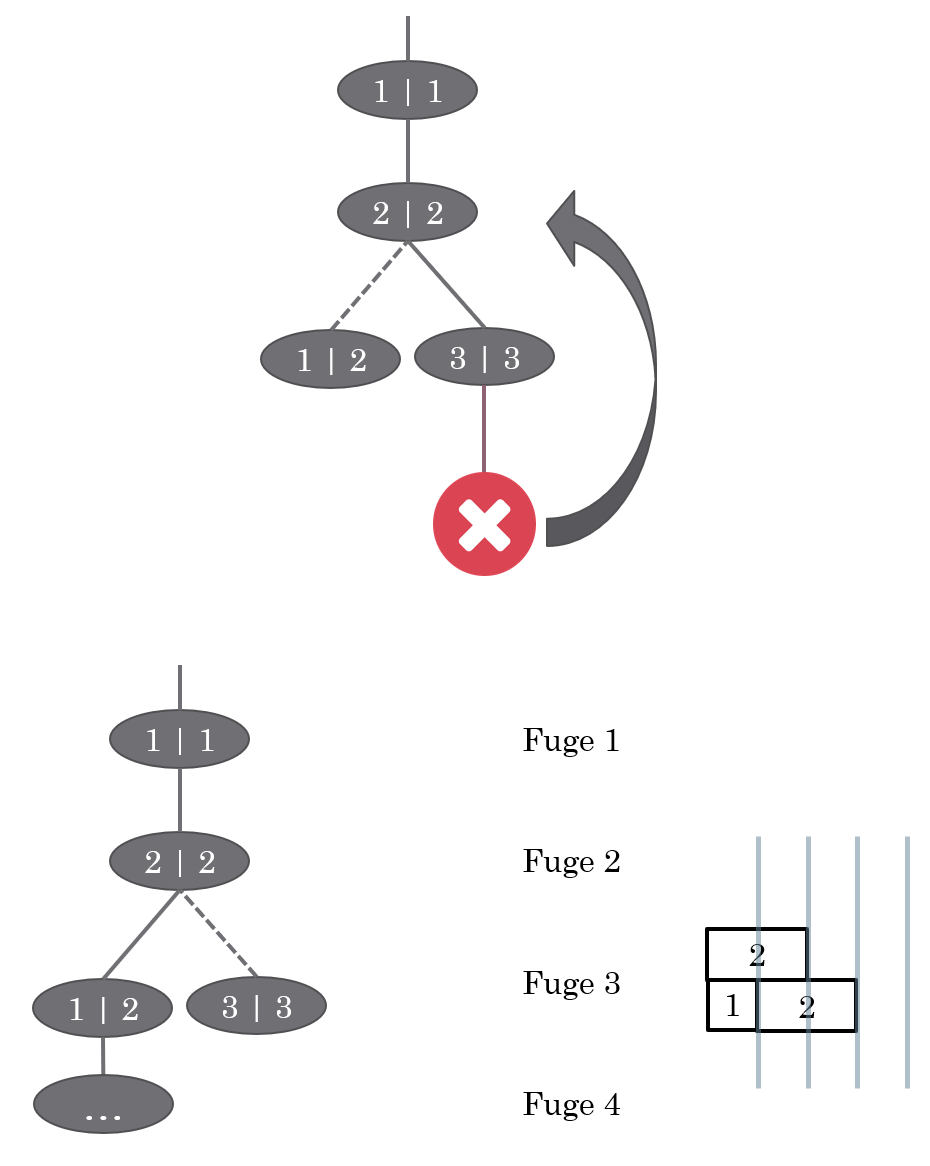
\includegraphics[width=1\linewidth]{Bilder/Aufgabe1/Backtracking_03_04.png}
    % TODO: Quelle für Trial and error Prinzip
    \caption{Nach dem "Trial and error" Prinzip wird beim Backtracking zur letzten Entscheidung zurückgegangen (oberes Bild) und ein anderes Klötzchen ausgewählt (unteres Bild). Dann wird mit dem Algorithmus fortgefahren.}
\end{figure}

Damit ist der grundlegende Algorithmus vollständig.
\subsection{Implementierung}
Das Programm wurde in der Sprache C\# als Konsolen Applikation mit dem .NET Framework 4.7.1 geschrieben.
Das am Ende des Kapitels in Abbildung 21 gezeigte Klassendiagramm zeigt die Grundstruktur des Programms.
\\[0.4cm]
Im Folgenden soll nur die Implementierung der für den Algorithmus wichtigsten Methode erklärt werden. Auf der beigelegten CD befindet sich zusätzlich eine vollständige Dokumentation aller Methoden und Attribute einmal in Form eines PDFs und einer HTML-Website.
\\[0.4cm]
Die Klasse \code{WallBuilder} ist für den Algorithmus die wichtigste Klasse. Sie baut die Mauer. Die für diesen Vorgang verantwortliche Methode ist \code{FillNextGap} (siehe Abbildung 20), die als Eingabeparameter einen Integer \code{nextGap}, ein \code{Wall} Objekt \code{curWall} und einen weiteren Integer \code{freeGaps} erwartet und ein Objekt der Klasse \code{Wall} zurückgibt.
\\[0.4cm]
Die Methode ist \textbf{direkt Rekursiv} und teilt somit die Problemstellung, eine komplette Mauer zu bauen in mehrere kleinere Probleme auf. Diese sind für die jeweils nächste Fuge einen Klotz zu finden, der sie besetzt.
\\[0.4cm]
% TODO: Quelle für LINQ
Als erstes wird mit der Abbruchbedingung in Zeile 4 kontrolliert, ob die Mauer vollständig gebaut ist. Durch das Programmiermodell \textbf{LINQ} wird überprüft ob die Summe aller platzierten Klötzchen jedes \code{Row} Objekts der übergebenen \code{Wall} Instanz \code{curWall}, mit der Länge einer vollständigen Mauer übereinstimmt.
Ist die Abbruchbedingung \code{true}, so kommt es zu einem Rekursionsende und das fertige \code{Wall} Objekt wird zurückgegeben.
\\[0.4cm]
% TODO: Quelle für Reference-Type
Ansonsten wird das übergebene \code{Wall} Objekt 'kopiert', denn es ist sehr wichtig, dass am übergebenen \code{curWall} Objekt nichts geändert wird. Objekte der Klassen \code{Wall} und \code{Row} sind nämlich sogenannte Referenz Typen (engl. Reference Types). Anders als bei Werte Typen (engl. Value Types), bei denen bei einer erneuten Zuweisung der gespeicherte Wert kopiert und die Variable dann auf diesen kopierten Wert verweist, wird bei einer erneuten Zuweisung eines Referenz Typs \textbf{nur der Verweis} (engl. Pointer) \textbf{kopiert}. Die Variable greift jedoch auf das \textbf{gleiche Objekt im Systemspeicher} zu wie die vorherige Variable.

Dies hätte zu Folge, dass wenn wir an dem übergebenen \code{Wall} Objekt zu späterem Zeitpunkt irgendwelche Änderungen vornehmen, sich auch das \code{Wall} Objekt der Aufrufer-Methode ändert. Dies würde das Backtracking erheblich erschweren, da wir nicht mehr auf den \textbf{vorherigen Zustand} der Mauer \textbf{vor einer Klötzchen Entscheidung} zurückgreifen könnten.
\\[0.4cm]
In Zeile 10 bis 14 wird dann die, für den aktuellen Schritt, zu befüllende Fugenposition gewählt. Der Parameter \code{nextGap} beschreibt also die \textbf{zuletzt gefüllte Fuge}.

Es wird überprüft, ob es nach \code{nextGap} überhaupt noch eine Fuge gibt. Ist dem so wird die Variable \code{nextGapPos} mit dem Wert \code{nextGap + 1}, also der Position der nächsten Fuge, initialisiert. Es kann jedoch auch sein, dass die Mauer schon am Ende angelangt ist und im letzten Schritt bereits die letzte 'Fugenposition' und damit ist hierbei das Ende der Mauer gemeint, gefüllt wurde (siehe Abbildung 19). Wichtig hierbei ist, dass dies nicht direkt heißt, dass die Mauer fertig ist. Es muss nämlich jede andere Reihe auch noch die letzte 'Fuge' erreichen.
\begin{figure}[H]
    \centering
    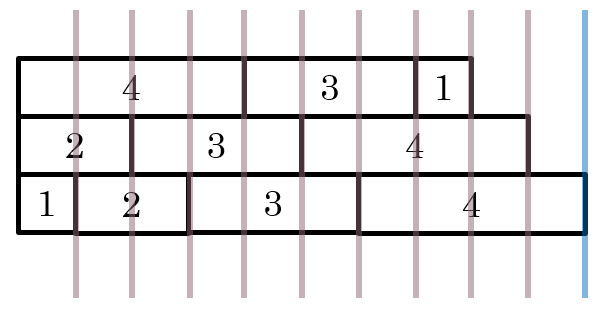
\includegraphics[width=.6\linewidth]{Bilder/Aufgabe1/Code_Algorithmus_01.png}
    \caption{Bei dieser Mauer von $n = 4$ hat die unterste Reihe die letzte 'Fugenposition' bereits gefüllt. Diese End-'Fuge' darf und muss jedoch mehrmals besetzt werden, um jede Reihe abzuschließen.}
\end{figure}
Deshalb wird in diesem Fall die Variable \code{nextGapPos} mit dem gleichen Wert wie \code{nextGap} initialisiert.
\\[0.4cm]
% TODO: QUELLE für LINQ
Im nächsten Ausdruck, der sich von Zeile 17 bis 19 erstreckt, werden wieder mittels \textbf{LINQ} alle \code{Row} Objekte der aktuellen \code{Wall} Instanz, die durch ein noch verfügbares Klötzchen die gewünschte Fugenposition befüllen können, in einem Array gesammelt.
\\[0.4cm]
Von Zeile 22 bis 34 wird nun geprüft, ob es keine einzige Reihe gibt, die die nächste Fuge besetzen kann. Hier wird auf den Sonderfall geschaut, dass der Parameter \code{freeGaps} größer als 0 ist. Dies kann nämlich der Fall sein, wenn $n$ \textbf{ungerade} ist. Bei ungeraden $n$ kann es ja zu vollständigen Mauern kommen, \textbf{ohne}, dass \textbf{alle} Fugen besetzt sind. In der Tat kann man auch relativ einfach ausrechnen, wie viele Fugen für ein ungerades $n$ frei bleiben können (siehe Methode \code{CalculateWallProperties} der Klasse \code{WallBuilder}. Somit kann es passieren, dass wenn kein Klötzchen in keiner Reihe zum Besetzen einer freien Fuge gefunden wurde und der 'freie Fugen Puffer' der aktuellen Mauer noch größer als 0 ist, dass diese freie Fuge \textbf{nicht besetzt} und einfach \textbf{übersprungen} werden kann.
Deshalb findet in Zeile 26, wenn \code{freeGaps} noch größere als 0 ist, einfach der rekursive Aufruf statt mit dem \code{freeGaps} Parameter um 1 verringert. Der Rückgabewert dieses rekursiven Aufrufs wird in der Variable \code{result} gespeichert. Ist \code{result} ein \code{Wall} Objekt, wird dieses weiter zurückgegeben, ansonsten wird der restliche Code bis zum Rekursionsende in Zeile 51 ausgeführt.
Tritt der Sonderfall \code{freeGaps > 0} nicht ein wird \code{null} zurückgegeben.
\\[0.4cm]
In Zeile 37 wird das Array der \code{Row} Objekte, die die nächste Fuge füllen können nach ihrer \code{RowSum} sortiert. Mit \code{RowSum} ist hierbei einfach die Summe aller in der Reihe platzierten Klötzchen gemeint.
Nach dem Sortieren, ist das erste Objekt des \code{possibleRows} Arrays also die \textbf{kürzeste Reihe} und das letzte Objekt die bereits \textbf{längste Reihe}.
\\[0.4cm]
In der For-Schleife von Zeile 40 bis 48 werden nun die \code{Row} Objekte des \code{possibleRows} Array einzeln iteriert.
Zuerst wird in Zeile 42 das Klötzchen platziert, dass die gesuchte Fuge füllt. (Das Klötzchen wurde in der vorher aufgerufenen Methode \code{ContainsPossibleRowSum} der Klasse \code{WallBuilder} herausgefiltert.)

Danach kommt ein rekursive Aufruf, dessen Rückgabewert in der lokalen Variabel \code{result} gespeichert wird. In der Abbruchbedingung von Zeile 44 wird wieder überprüft, ob \code{result} ein \code{Wall} Objekt ist. Ist dies der Fall, wird es weiter zurückgegeben.

Ist im Gegensatz dazu \code{result} gleich \code{null}, heißt das, dass mit dieser Klötzchen-Entscheidung keine fertige Mauer gebaut werden konnte und deshalb bis zu dieser Entscheidung zurückgegangen wurde, um dort ein anderes Klötzchen zu wählen (\textbf{Backtracking}).

Deshalb wird das zuvor platzierte Klötzchen des aktuellen \code{Row} Objekts in Zeile 47 wieder entfernt.

Gibt es danach noch weitere \code{Row} Objekte im \code{possibleRows} Array, wird die Schleife mit dem nächsten \code{Row} Objekt durchlaufen.
\\[0.4cm]
Als letzte Anweisung der Methode wird mit einem Rekursionsende \code{null} zurückgegeben.
\begin{figure}[H]
    \centering
    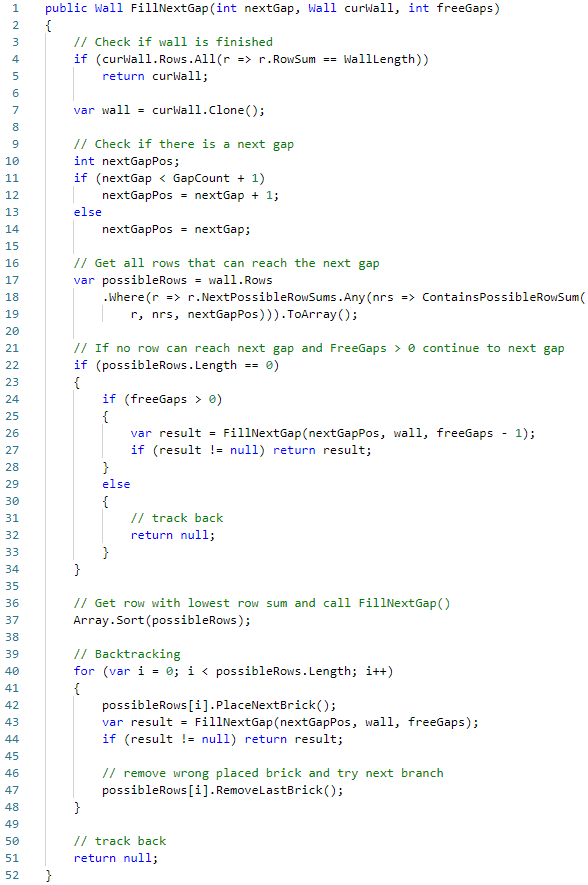
\includegraphics[width=.86\linewidth]{Bilder/Aufgabe1/Code.png}
    \caption{Quellcode der Methode \code{FillNextGap} der Klasse \code{WallBuilder}.}
\end{figure}
\begin{figure}[H]
    \centering
    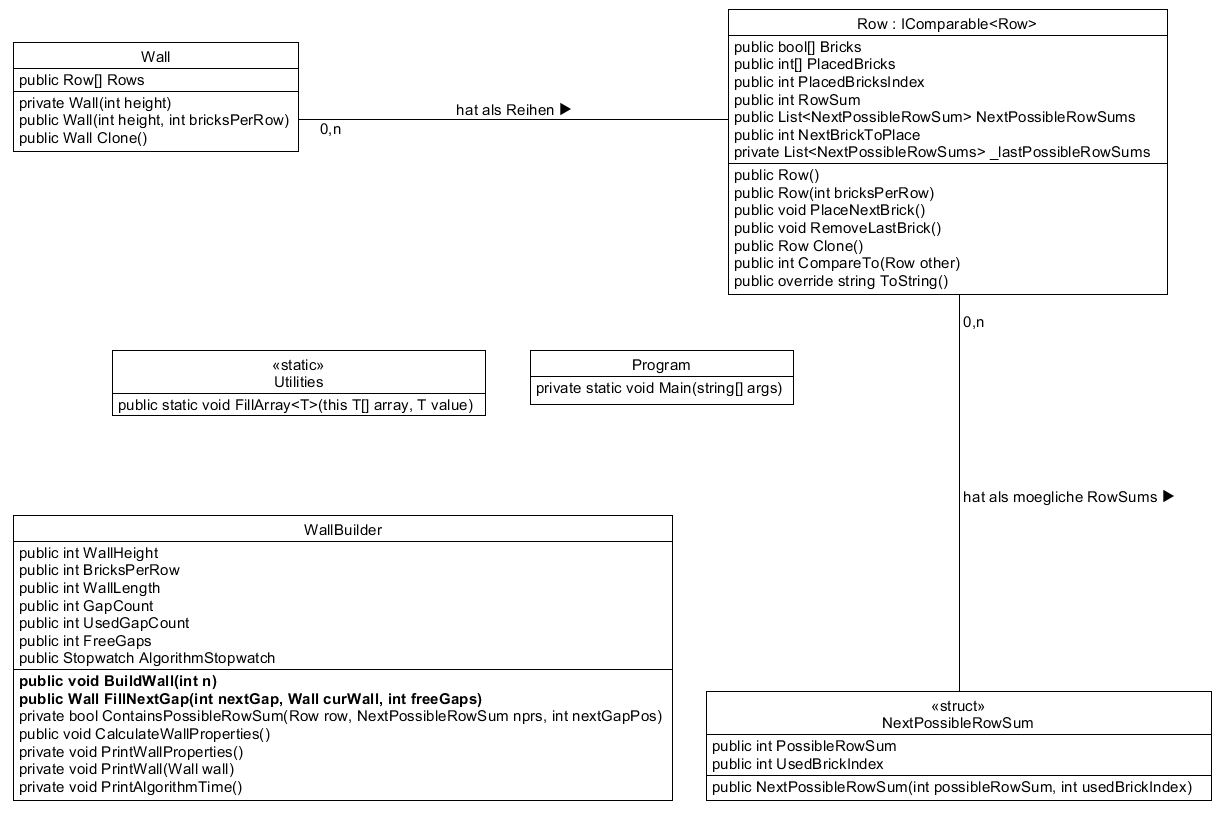
\includegraphics[width=.925\linewidth]{Bilder/Aufgabe1/Klassendiagramm.png}
    \caption{Erweitertes Klassendigramm des Programms. Die wichtigsten zwei Methoden des Algorithmus wurden in der Klasse \code{WallBuilder} hervorgehoben.}
\end{figure}

\subsection{Optimierungsmöglichkeiten}

\subsection{Beispiele}


%===================================================================================
%-------------------------------- AUFGABE 3 ----------------------------------------
%===================================================================================

\newpage
\section{AUFGABE 3 - "Quo vadis, Quax?"}



\subsection{Aufgabenstellung}

\subsection{Lösungsidee}

\subsection{Teilaufgabe (a)}

\subsection{Teilaufgabe (b)}

\subsection{Teilaufgabe (c)}
\subsubsection{Implementierung}
\subsubsection{Optimierungsmöglichkeiten}
\subsubsection{Beispiele}

\subsection{Teilaufgabe (d)}


%===================================================================================
%---------------------------------- FAZIT ------------------------------------------
%===================================================================================

\newpage
\section{FAZIT}



Lorem ipsum dolor sit amet, consectetur adipiscing elit. Sed tempus consectetur lorem, imperdiet dignissim est auctor a. Vivamus convallis, leo et iaculis egestas, nunc massa porttitor tellus, id faucibus urna justo eget massa. Praesent quis feugiat odio. Nullam quis mattis enim. Fusce volutpat odio in enim sodales venenatis. Mauris consequat.

%===================================================================================
%--------------------------- ABBILDUNGSVERZEICHNIS ---------------------------------
%===================================================================================

\newpage
\section{ABBILDUNGSVERZEICHNIS}
Alle enthaltenen Abbildungen wurden mithilfe von folgenden Tools selbstständig erstellt:
\begin{itemize}
\item Microsoft PowerPoint
\item Grafikrechner - GeoGebra
\item UMLet
\item Adobe Photoshop CC 2018 
\end{itemize}

%===================================================================================
%--------------------------- LITERATURVERZEICHNIS ----------------------------------
%===================================================================================

\newpage
\section{LITERATURVERZEICHNIS}

\begingroup
\renewcommand{\section}[2]{}%
\begin{large}
\textbf{Buchquellen:}
\end{large}

\begin{thebibliography}{9}

    \bibitem{lamport94}
      Leslie Lamport,
      \textit{\LaTeX: a document preparation system},
      Addison Wesley, Massachusetts,
      2nd edition,
      1994.
      \bibitem{lamport91}
      Leslie Lamport,
      \textit{\LaTeX: a document preparation system},
      Addison Wesley, Massachusetts,
      2nd edition,
      1994.
      \bibitem{lamport97}
      Leslie Lamport,
      \textit{\LaTeX: a document preparation system},
      Addison Wesley, Massachusetts,
      2nd edition,
      1994.

\end{thebibliography}

\vspace{1cm}

\begin{large}
\textbf{PDF-Scans:}
\end{large}

\begin{thebibliography}{9}

    \bibitem{bwinf_runde1_ergebnis}
      Leslie Lamport,
      \textit{\LaTeX: a document preparation system},
      Addison Wesley, Massachusetts,
      2nd edition,
      1994.
  	\bibitem{bwinf_runde2_ergebnis}
      Leslie Lamport,
      \textit{\LaTeX: a document preparation system},
      Addison Wesley, Massachusetts,
      2nd edition,
      1994.

\end{thebibliography}

\vspace{1cm}

\begin{large}
\textbf{Internetquellen:}
\end{large}

\begin{thebibliography}{9}

    \bibitem{lamport94}
      Leslie Lamport,
      \textit{\LaTeX: a document preparation system},
      Addison Wesley, Massachusetts,
      2nd edition,
      1994.
      \bibitem{lamport91}
      Leslie Lamport,
      \textit{\LaTeX: a document preparation system},
      Addison Wesley, Massachusetts,
      2nd edition,
      1994.
      \bibitem{lamport97}
      Leslie Lamport,
      \textit{\LaTeX: a document preparation system},
      Addison Wesley, Massachusetts,
      2nd edition,
      1994.

\end{thebibliography}

\endgroup

%===================================================================================
%--------------------------- CD-VERZEICHNIS ----------------------------------
%===================================================================================

\newpage
\section{CD-VERZEICHNIS}

%===================================================================================
%--------------------------- ANHANG ----------------------------------
%===================================================================================

\newpage
\section{ANHANG}
\subsection{Aufgabe 1}
\subsubsection{Quelltext}
\subsubsection{Dokumentationen}
\subsubsection{Installationshinweise}

\subsection{Aufgabe 3}
\subsubsection{Quelltext}
\subsubsection{Installationshinweise}

%===================================================================================
%------------------------- ERKLÄRUNG DES VERFASSERS --------------------------------
%===================================================================================

\newpage
\section{ERKLÄRUNG DES VERFASSERS}



Lorem ipsum dolor sit amet, consectetur adipiscing elit. Sed tempus consectetur lorem, imperdiet dignissim est auctor a. Vivamus convallis, leo et iaculis egestas, nunc massa porttitor tellus, id faucibus urna justo eget massa. Praesent quis feugiat odio. Nullam quis mattis enim. Fusce volutpat odio in enim sodales venenatis. Mauris consequat.

\begin{figure}[H]
    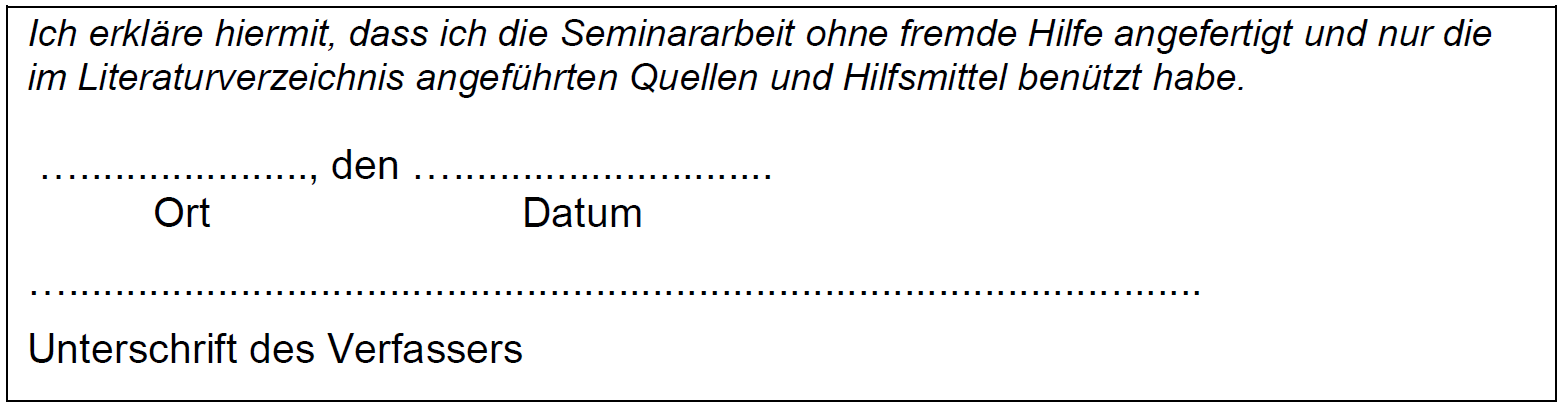
\includegraphics[width=\linewidth]{Bilder/Sonstiges/ErklaerungDesVerfassers.png}
\end{figure}

\end{document}